\section{Design}
\label{sec:design}
To create ClouDJ, we implemented the design described 
in subsections \ref{sec:architecture} and \ref{sec:execution} 
by integrating Google App Engine. 
Figure \ref{fig:arch} depicts the overall system.

\begin{figure*}[ht]
\centering
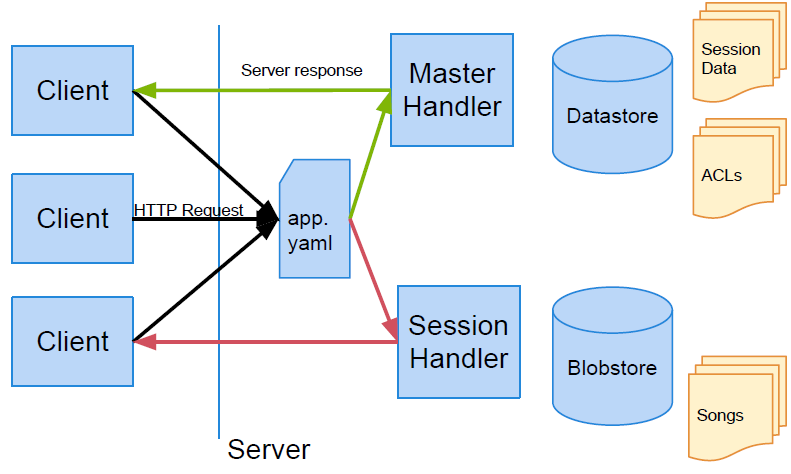
\includegraphics[width=160mm]{architecture.png}
\caption{The system architecture.}
\label{fig:arch}
\end{figure*}

\subsection{Architecture}
\label{sec:architecture}
There are three major roles in our system: 
the master handler, session handler, and client. Clients own 
and store music, can share their music with others 
and can listen to music shared by others. The master handler provides 
access control, starts sessions for users who want to host, and
acts as a liaison between the clients and session servers. The session 
handler is in charge of handling synchronization messages between clients
and serving content.

\subsubsection{Front End}
\label{sec:frontend}
A session is an abstraction in which multiple users 
may listen to one song that is hosted by a single user. 
Our front end (client) application allows a user to either 
create a session and become a host, or join an existing 
session and become a listener. When acting as a host, 
a user may add songs from the session playlist, 
play or pause the current song, and skip to the next song. 
When acting as a listener, the user has 
no control over what song is being played. Users can 
see all sessions that they are able to join. Only 
members of a user's access control list (ACL) may 
see or join any session in which that user is a host.

The client has access to its user's music and playlists and 
also keeps track of data such as the user's current 
session and the user's potential sessions (sessions 
this user can access). For the current session, the 
client keeps track of the current session key and relevant song information. 
For the potential sessions, the client keeps the host, 
session key, and currently playing song.

\subsubsection{Back End}
\label{sec:backend}
The backend infrastructure is more complicated than 
the frontend. The master server keeps track of users 
currently online, user ACLs, and user membership lists 
(ACLs it is a member of). It also is responsible for 
maintaining a session table, a table that maps host 
users to sessions (this is a one-to-one mapping). 
When a client logs on, the master server informs each 
session associated to a host on the client's 
membership list that this client is a potential listener.

The session handler is the workhorse of the system. It 
services requests for sessions it is in charge of by 
routing data from the host client to relevant clients 
(listeners). It maintains the list of listeners and 
potential listeners. A potential listener is a client 
who could listen to this session, but is currently not. 
In other words, these are the clients on the host client's 
ACL that are logged in but not listening to this 
session. Session servers also take care of session 
cleanup when a session ends (or fails). 

\subsubsection{Storage}
\label{sec:storage}
Certain information is stored on the server in the Datastore and Blobstore.
Datastore holds session data and ACLs. 
Session data includes session meta data (session key, host, listeners), 
and session state (current song, song play or pause flag, session ended flag, 
timestamp of last play/next message). This information is used to coordinate
sessions among different clients. The ACLs keeps track of the potential
sessions and potential listeners for each user. Potential listeners are 
users who can listen to a session hosted by a given user and potential sessions
are sessions the user can join. Blobstore is only used 
to store song data in our application. When a session ends, the songs are deleted 
from the blobstore.

\subsection{Execution Flow}
\label{sec:execution}
As shown in Figure~\ref{fig:arch}, the general execution of the ClouDJ application
is as as follows:
\begin{enumerate}
  \item The client contacts the server
  \item The server performs executes the handler based on the request
  \item The handler runs and propagates updates to session participants
  \item The client receives the server response and performs actions 
\end{enumerate}

In sections \ref{sec:joinSession} and \ref{sec:playSession}, we discuss
session creation, joining and leaving sessions, and updating sessions.


\subsubsection{Creating, Joining, and Leaving a Session}
\label{sec:joinSession}
Sessions are created when a client contacts the master 
handler about hosting a new session. The master handler 
then creates a new session in the datastore and responds to the client, 
which updates its current session information. 
Clients may join sessions by contacting the master 
handler with the session key of the session they wish to join. 
The master handler updates the session information in the datastore
and notifies everyone in the session of the new listener. 
After a session is established, the client no longer communicates 
with the master handler. When a user leaves a session, the client
contacts the session handler telling it to remove itself from from
the listener list if it is not the host. If it is the host the
session handler notifies all listeners that the session has ended and 
removes the session and corresponding song data from the datastore
and blobstore.

\subsubsection{Updating Sessions}
\label{sec:playSession}
Hosts may update the sessions using several types of messages: ``upload'',
``play,'' ``pause,'' and ``next,''. Songs are added to the session when 
the host client contacts the session handler with an ``upload'' message, 
indicating that it wants to add a song to the playlist. The session 
handler forwards the song to the blobstore and retrieves the corresponding 
blob key, which is used when requesting the song for playback. The session
handler then updates the session playlist in the datastore and sends the 
blob key to all clients in the session. The clients then fetch the song 
from the blobstore. 

Not surprisingly, the ``play'', ``pause,'' and ``next'' messages 
indicate when the host wants to unpause, pause, and skip the current song, respectively.
The host sends these control messages to the session handler, which updates
the session in the datastore and then propagates the message to all session
participants. The clients then peform the appropriate action. We elaborate on
playback synchronization among clients in Section~\ref{sec:sync}.